\documentclass[11pt]{article}
\usepackage[margin=0.8in]{geometry}
\usepackage{graphicx}
\usepackage{amsmath,amssymb}
\usepackage[T1]{fontenc}
\usepackage{lmodern}
\begin{document}
\begin{center}
{\Large Adaptive batching: scalar cancellation and fixed roots}\\[5pt]
{\small Formal review packet, 2 November 2026}
\end{center}

\noindent\textbf{Claim.} Over every field $F$, the challenge-dependent errors
$e_0(\rho)=-\rho$ and $e_1(\rho)=1$ are nonzero as a pair and satisfy
$e_0(\rho)+\rho e_1(\rho)=0$ for every $\rho$. For fixed
$(a,b)\ne(0,0)$ over a finite field, the set
$\{\rho\in F:a+\rho b=0\}$ has cardinality at most one.

\begin{center}
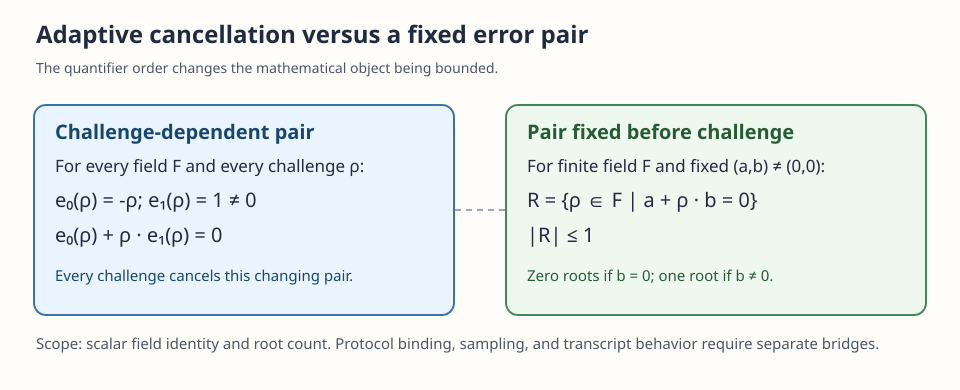
\includegraphics[width=\linewidth]{quantifier-boundary.png}
\end{center}

\noindent\textbf{Evidence.} The blind mathematical review checks both
claims directly, enumerates $\mathbb F_2$, and exhibits the zero-pair and
$\mathbb Z/4\mathbb Z$ boundary cases. The independent source review checks
the frozen target and source against the named Lean declaration at commit
\texttt{8a9daca52daa3c121424bad54c0260cfaedb33b2}. It found and
resolved an omitted binder in an earlier head. The exact machine status,
receipt identity, and transitive axiom result are recorded below.

\noindent\textbf{Machine status.} Hosted run 41488317240 passed on the merge
of main \texttt{63690685} and proof head \texttt{8a9daca5}. Its named receipt
for \texttt{adaptive\_rlc\_cancellation} reports \texttt{machine\_verified},
successful build and axiom audit, and no forbidden constructs. The elaborated
type retains both field quantifiers, the finite-field enumeration, and the
nonzero fixed-pair premise. Its transitive axioms are \texttt{propext},
\texttt{Classical.choice}, and \texttt{Quot.sound}; the workspace audit counted
1,091 theorems with standard axioms only. The pre/post dependency-pin receipts
are byte-identical. The hosted Lean/Lake binaries were not independently
rechecked.

\noindent\textbf{Publication gate.} The proof PR remains open because two
unrelated DREG supersession harness checks failed on the tested merge tree.
The repair is separately proposed in PR 2973; the proof must pass its own
current-head checks after that repair before merging.

\noindent\textbf{Review process.} Both reviewers recorded their reads and
scoped verdicts. The repository independence checker rejected this round's
prewritten Markdown plan because it requires a YAML \texttt{review\_plan}
block. This procedural check remains open; its failure is not a Lean or
mathematical counterexample.


\noindent\textbf{Scope.} The theorem concerns a scalar field identity and a
univariate linear root count. A probability statement additionally needs a
specified challenge distribution and independence from the fixed pair.
Applying the identity to a batching protocol needs a verified mapping from
protocol errors and acceptance to this equation, including transcript and
binding behavior. No protocol-security or performance claim is derived here.

\noindent\textbf{Review artifacts.} The source and blind reports, frozen
review plan, current-head machine receipt, and source hashes accompany this
PDF in the archival packet. The diagram is rendered from the adjacent SVG.

\end{document}
